\documentclass[final,t]{beamer}
\mode<presentation>{\usetheme{Purdue}}

\usepackage{natbib,url}
\usepackage{multicol}
\usepackage{geometry}
\usepackage{multirow}
\usepackage{rotating}

%% Levi added (below)
% \usepackage{times}
% \usepackage{tikz}
% \usetikzlibrary{shapes,arrows}
% \usepackage{tikz-dependency}
%% Levi added (above)

\usepackage{enumerate}
\usepackage{color}
\usepackage{xcolor}

\definecolor{light-gray}{gray}{0.9}

\usepackage[orientation=portrait,size=a1,scale=1]{beamerposter}
\usepackage{gb4e}

\title[]{IUCL: Combining Information Sources for SemEval Task 5}
\author[]{Alex Rudnick, Levi King, Can Liu, Markus Dickinson, Sandra K\"ubler}
\institute[]{Indiana University}
\date[]{XX August 2014}

\begin{document}
\begin{frame}{}
  \begin{columns}[t]
    \begin{column}{.5\linewidth}

\begin{block}{Approach}

  \textbf{Language-independent approach:} make use of rich L2 context,
  along with proposed fragment translations

  \medskip

  % \begin{enumerate}
  % \item Model transfer knowledge between L1 \& L2: look up candidate
  %   translations for L1 fragment
  % \item Model facts about L2 syntax: score candidate translations via
  %   L2 LM
  % \item Model L2 collocational tendencies: score translations via
  %   dependency-driven word similarity (\textit{SIM})
  % \item Weight each source of information (\#1--\#3) in log-linear
  %   model to obtain final $n$-best list
  % \end{enumerate}

%  $\Rightarrow$ Language-independent approach

  % trim=left bottom right top, clip
  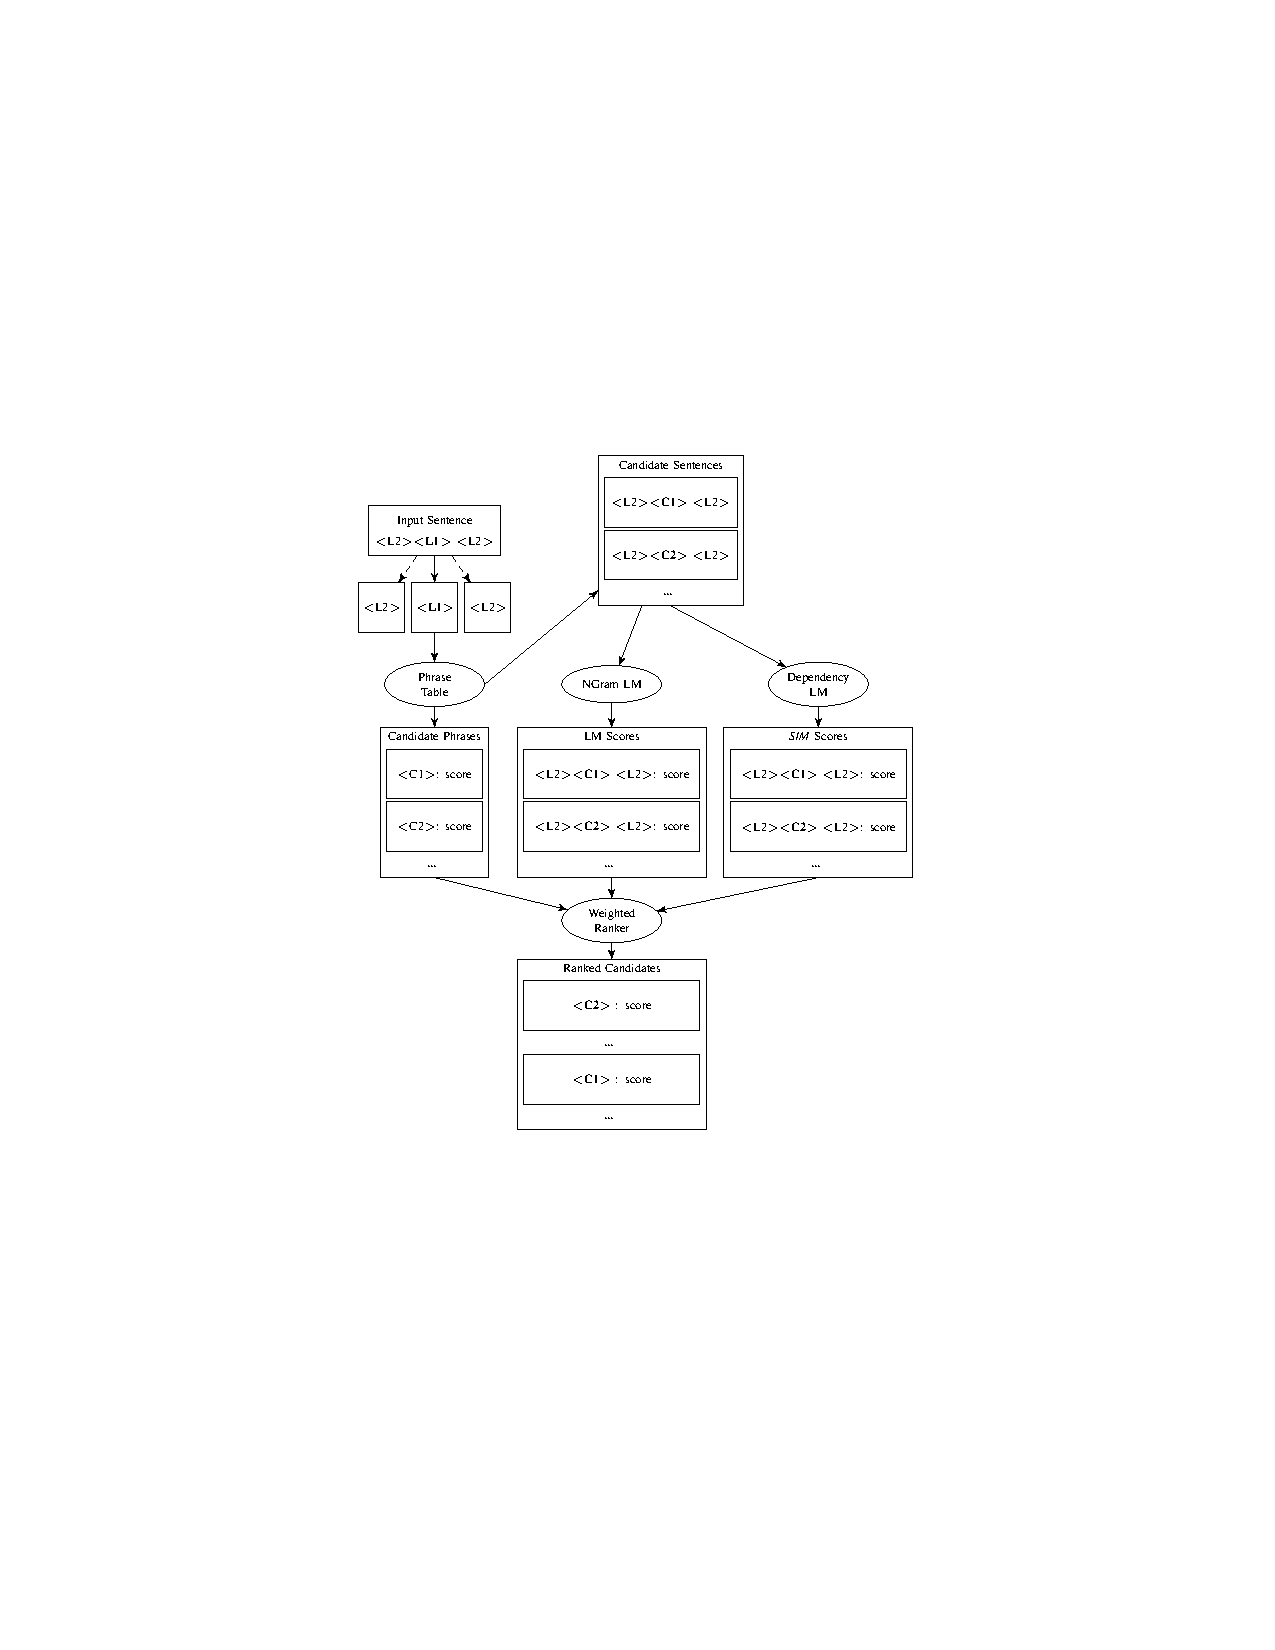
\includegraphics[width=.9\textwidth]{flowchart/chart}

\end{block}

\begin{block}{Steps in the pipeline}
  \begin{enumerate}
  \item \textbf{Phrase table}: 
    %Model L1$\mapsto$L2 transfer knowledge:
    look up candidate translations for L1 fragment
  \item \textbf{L2 ngram LM}: score candidate translations (L2 syntax)
  \item \textbf{Dependency-driven word similarity (\textit{SIM})}:
    score translations % (L2 collocations)
  \item \textbf{Weighted ranker}: weight \#1--\#3 in log-linear model
    to obtain $n$-best list
  \end{enumerate}
\end{block}

%%% Begin Levi's flowchart (currently doesn't in the poster, but works elsewhere!)
% Define block styles
%\tikzstyle{block} = [rectangle, draw, text width=10em, text centered, minimum height=4em]
%\tikzstyle{line} = [draw, -latex']
%\tikzstyle{cloud} = [draw, ellipse, minimum height=3em,  text width=5em, text centered,]
%
%\begin{figure}
%\begin{center}
%\tiny
%\begin{tikzpicture}[node distance = 1.3cm]
%    %nodes
%    \node [block, node distance=2.5cm] (input) {Input Sentence \\ \smallskip \textless L2\textgreater  \textbf{\textless L1\textgreater } \textless L2\textgreater };%Na
%    \node [block, below of=input, text width=3em] (TargetPhrase) {\textbf{\textless L1\textgreater }};%Nb2
%    \node [block, node distance=.9cm, left of=TargetPhrase, text width=3em] (SentBegin) {\textless L2\textgreater };%Nb1
%    \node [block, node distance=.9cm, right of=TargetPhrase, text width=3em] (SentEnd) {\textless L2\textgreater };%Nb3
%	\node [cloud, below of=TargetPhrase] (PhraseTable) {Phrase Table};%Nc
%	\node [block, text width=8em, node distance=2cm, below of=PhraseTable] (PTOutput) {Candidate Phrases \\ \smallskip
%		\begin{tikzpicture}[node distance = .7cm, auto]
%			\node [block, text width=7em, node distance=.7cm] (PTOC1) {\textless C1\textgreater  : score}; %Nd1
%		\end{tikzpicture}
%		\begin{tikzpicture}[node distance = .7cm, auto]
%			\node [block, text width=7em, below of=PTOC1] (PTOC2) {\textless C2\textgreater  : score}; %Nd2
%		\end{tikzpicture} \\ \textbf{...} \smallskip};%Nd
%	\node [block, text width=11em, node distance=4cm, right of=input] (CandidateSents) {Candidate Sentences \\ \smallskip
%		\begin{tikzpicture}[node distance=.7cm, auto]
%			\node [block, node distance=1.3cm] (CS1) {\textless L2\textgreater  \textbf{\textless C1\textgreater } \textless L2\textgreater }; %Ne1
%		\end{tikzpicture}
%		\begin{tikzpicture}[node distance = .7cm, auto]
%			\node [block, below of=CS1] (CS2) {\textless L2\textgreater  \textbf{\textless C2\textgreater } \textless L2\textgreater }; %Ne2
%		\end{tikzpicture} \\ \textbf{...} \smallskip};%Ne
%	\node [cloud, right of=PhraseTable, node distance=3cm] (NGramLM) {NGram LM};%Nf
%	\node [cloud, right of=NGramLM, node distance=3.5cm] (DependencyModel) {Dependency LM}; %Nh
%	\node [block, text width=14.5em, node distance=2cm, below of=NGramLM] (NLMOutput) {LM Scores \\ \smallskip
%		\begin{tikzpicture}[node distance = .7cm, auto]
%			\node [block, text width=13.5em, node distance=.7cm] (NLMO1) {\textless L2\textgreater  \textbf{\textless C1\textgreater } \textless L2\textgreater  : score}; %Ng1
%		\end{tikzpicture}
%		\begin{tikzpicture}[node distance = .7cm, auto]
%			\node [block, text width=13.5em, below of=NLMO1] (NLMO2) {\textless L2\textgreater  \textbf{\textless C2\textgreater } \textless L2\textgreater  : score}; %Ng2
%		\end{tikzpicture} \\ \textbf{...} \smallskip};%Ng
%	\node [block, text width=14.5em, node distance=2cm, below of=DependencyModel] (DMOutput) {\textit{SIM} Scores \\ \smallskip
%		\begin{tikzpicture}[node distance = .7cm, auto]
%			\node [block, text width=13.5em, node distance=.7cm] (DMO1) {\textless L2\textgreater  \textbf{\textless C1\textgreater } \textless L2\textgreater  : score}; %Ng1
%		\end{tikzpicture}
%		\begin{tikzpicture}[node distance = .7cm, auto]
%			\node [block, text width=13.5em, below of=DMO1] (DMO2) {\textless L2\textgreater  \textbf{\textless C2\textgreater } \textless L2\textgreater  : score}; %Ng2
%		\end{tikzpicture} \\ \textbf{...} \smallskip};%Ng	
%	\node [cloud, below of=NLMOutput, node distance=2cm] (Ranker) {Weighted Ranker}; %Nj
%	\node [block, text width=14.5em, node distance=2.1cm, below of=Ranker] (ROutput) {Ranked Candidates \\ \smallskip
%		\begin{tikzpicture}[node distance = .7cm, auto]
%			\node [block, text width=13.5em, node distance=.7cm] (DMO1) {\textbf{\textless C2\textgreater } : score}; %Ng1
%		\end{tikzpicture}
%		\textbf{...} \smallskip \\
%		\begin{tikzpicture}[node distance = .7cm, auto]
%			\node [block, text width=13.5em, below of=DMO1] (DMO2) {\textbf{\textless C1\textgreater } : score}; %Ng2
%		\end{tikzpicture} \\ \textbf{...} \smallskip};%Ng	
%	%paths
%	\path [line] (input) -- (TargetPhrase);%Pa
%	\path [line] (TargetPhrase) -- (PhraseTable);%Pb
%	\path [line, dashed] (input) -- (SentBegin);
%	\path [line, dashed] (input) -- (SentEnd);
%	\path [line] (PhraseTable) -- (PTOutput);%Pc1
%	\path [line] (PhraseTable.east) -- (CandidateSents);%Pc2
%	\path [line] (CandidateSents) -- (NGramLM); %Pe1
%	\path [line] (CandidateSents.south) -- (DependencyModel); %Pe2
%	\path [line] (NGramLM) -- (NLMOutput); %Pf
%	\path [line] (DependencyModel) -- (DMOutput); %Ph
%	\path [line] (PTOutput.south) -- (Ranker); %Pd
%	\path [line] (NLMOutput) -- (Ranker); %Pg
%	\path [line] (DMOutput.south) -- (Ranker); %Pi
%	\path [line] (Ranker) -- (ROutput); %Pi
%\end{tikzpicture}
%\end{center}
%\caption{(Something about our approach....)}
%\label{fig:flowchart}
%\end{figure}
%%% End Levi's flowchart.

%\end{block}

%\end{column}

%\begin{columns}
%  \begin{column}{.5\linewidth}

\begin{block}{Results}

\begin{center}
  \textcolor{purple}{English-German (next-best: CNRC-run1)}
  %\begin{figure}[t]
  \begin{center}
  \begin{tabular}{|r|c|c|c|c|}
    \hline
    system & acc      & wordacc  & oofacc & oofwordacc \\
    \hline
    run2  &  0.665 & 0.722  &  0.806  & 0.857 \\
    SIM    &  0.647 & 0.706 & 0.800 & 0.852 \\
    next-best     &  0.657   & 0.717   & 0.834 & 0.868    \\
    \hline
  \end{tabular}
  \end{center}
%\caption{Scores on the test set for English-German; here next-best is CNRC-run1.}
%\label{fig:theresults-en-de}
%\end{figure}

  \textcolor{purple}{English-Spanish (best: UEdin-run2)}
%\begin{figure}[t]
  \begin{center}
  \begin{tabular}{|r|c|c|c|c|}
    \hline
    system & acc      & wordacc  & oofacc & oofwordacc \\
    \hline
    run2  &  0.633 & 0.72 & 0.781 & 0.847 \\
    SIM    &  0.359 &  0.482 & 0.462 & 0.607 \\
    best   &  0.755 & 0.827   & 0.920  & 0.944 \\
    \hline
  \end{tabular}
  \end{center}
%\caption{Scores on the test set for English-Spanish; here best is UEdin-run2.}
%\label{fig:theresults-en-es}
%\end{figure}

 \textcolor{purple}{French-English (best: UEdin-run1)}
%\begin{figure}[t]
  \begin{center}
  \begin{tabular}{|r|c|c|c|c|}
    \hline
    system & acc      & wordacc  & oofacc & oofwordacc \\
    \hline
    run2  & 0.545  & 0.682 & 0.691 & 0.800 \\
    SIM        &  0.549 & 0.687 & 0.693 & 0.800 \\
    best & 0.733 & 0.824 & 0.905 & 0.938 \\
    \hline
  \end{tabular}
  \end{center}
%\caption{Scores on the test set for French-English; here best is UEdin-run1.}
%\label{fig:theresults-fr-en}
%\end{figure}

  \textcolor{purple}{Dutch-English (best: UEdin-run1)}
%\begin{figure}[t]
  \begin{center}
  \begin{tabular}{|r|c|c|c|c|}
    \hline
    system & acc      & wordacc  & oofacc & oofwordacc \\
    \hline
    run2        &  0.544      &  0.679  & 0.634   & 0.753    \\
    SIM              &  0.540      &  0.676  & 0.635   & 0.753    \\
    best       &  0.575   & 0.692  & 0.733      &  0.811 \\
    \hline
  \end{tabular}
  \end{center}
%\caption{Scores on the test set for Dutch-English; here best is UEdin-run1.}
%\label{fig:theresults-nl-en}
%\end{figure}

\end{center}
\end{block}

\end{column}

\begin{column}{.47\linewidth}

\begin{block}{Data sources}

\begin{center}
\textcolor{purple}{Europarl}
\end{center}

\colorbox{white}{
\begin{minipage}{.85\linewidth}
\begin{itemize}
\item parallel corpus: proc.\ of European Parliament
\item used for L2 candidate generation
\item  used to generate phrase tables
\item small, clean, out of domain
\end{itemize}
\end{minipage}
}

\begin{center}
\textcolor{purple}{BabelNet}
\end{center}

\colorbox{white}{
\begin{minipage}{.85\linewidth}
\begin{itemize}
\item multilingual encyclopedic dictionary
\item used as L2 back-off 
\item look up translations for phrases \& sub-phrases
\end{itemize}
\end{minipage}
}

\begin{center}
\textcolor{purple}{Wikipedia}
\end{center}

\colorbox{white}{
\begin{minipage}{.85\linewidth}
\begin{itemize}
\item used for estimating collocational tendencies
\item size: 12-28M sentences
\item POS tagged \& dependency parsed (Stanford Parser)
\end{itemize}
\end{minipage}
}

\begin{center}
\textcolor{purple}{Google Books Syntactic N-grams}
\end{center}

\colorbox{white}{
\begin{minipage}{.85\linewidth}
\begin{itemize}
\item English only
\item additional training set for collocations tendencies
\item syntactic $n$-grams 

\end{itemize}
\end{minipage}
}

\end{block}

%  \end{column}
%\end{columns}

%\begin{column}{.47\linewidth}

%\begin{columns}
%\begin{column}{.48\linewidth}

\vspace{3ex}

\begin{block}{System Design}

\begin{center}
  \textcolor{purple}{1. Constructing Candidate Translations}
 \end{center}

 \colorbox{white}{
\begin{minipage}{.90\linewidth}
 \begin{itemize}
  \item build phrase tables using Moses
  \item during translation: look up source lg.\ phrase, \\
    \mbox{}\hspace{8em}extract all translations from phrase table\\[1ex]
  % \item back-offs: 1: construct ``synthetic phrase'' from sub-phrases
  % \item[] \mbox{}\hspace{4.1em} 2: look up phrase in BabelNet; estimate probs uniformly
  % \item back-off 3: look up phrase in Google Translate\\
  \item back-off: \begin{tabular}{cl}
       1: & construct ``synthetic phrase'' from sub-phrases\\
       2: & look up phrase in BabelNet; estimate probs uniformly\\
       3: & look up phrase in Google Translate\\
     \end{tabular}
  \end{itemize}
\end{minipage}
}
\vspace{1cm}


\begin{center}
  \textcolor{purple}{2. Scoring Candidate Translations via a L2 Language Model}
\end{center}
 
  \colorbox{white}{
\begin{minipage}{.90\linewidth}
 \begin{itemize}
  \item model the fit of phrase in context
  \item apply language model (KenLM); trained on Wikipedia data
  \end{itemize}
\end{minipage}
}
\vspace{1cm}

%\end{center}

%\end{block}

%\end{column}

%\begin{column}{.48\linewidth}

%\begin{block}{System Design}
%\begin{center}

\begin{center}
  \textcolor{purple}{3. Scoring Candidate Translations via Dependency-Based Word Similarity}
\end{center}

  \colorbox{white}{
\begin{minipage}{.90\linewidth}
  \begin{itemize}
  \item basic idea: use deeper, syntax-based information to estimate fit
    \begin{itemize}
    \item use adaptation of Lin's similarity metric
    \item similarity is summed over all words in translated phrase
    \end{itemize}
  \item use dependencies to \& from this word to context
    \begin{itemize}
    \item similarity based on head, dependent, and label of dependency 
    \item back-off: use POS instead of words
    \end{itemize}
  \item example: \\
    \textcolor{blue}{The suitcases disappeared after the $<$Aufgabe$>$ at the airport.}
    \begin{itemize}
    \item most frequent sense: \textcolor{blue}{Aufgabe = task}\\
    \item google: \textcolor{blue}{The suitcase had disappeared after posting at the airport.}
    \end{itemize}      
  \end{itemize}
\end{minipage}
}
\vspace{1cm}

\begin{center}
  \textcolor{purple}{4. Tuning Weights with MERT}
\end{center}

  \colorbox{white}{
\begin{minipage}{.90\linewidth}
  \begin{itemize}
  \item use long-linear model to combine scores from different information
  \item weights for different types of information estimated using ZMERT
  \item ZMERT optimized for BLEU scores
  \end{itemize}
\end{minipage}
}

\end{block}

\vspace{3ex}

\begin{block}{Conclusion}

\begin{itemize}
\item L2 language assistant based on language models
\item approach is language independent
\item uses syntactic information
\item but: syntactic information currently not helpful 

  Open Question: why isn't syntax helpful?  how could it be?
\end{itemize}

\end{block}


%    \end{column}
%  \end{columns}
\end{column}
\end{columns}


\end{frame}
\end{document}